\documentclass[12pt, oneside]{article}
\usepackage[letterpaper, margin=1in, headsep=0.5in]{geometry}
\usepackage[english]{babel}
\usepackage[utf8]{inputenc}
\usepackage{amsmath}
\usepackage{amsfonts}
\usepackage{amssymb}
\usepackage{tikz}
\usetikzlibrary{quotes, angles}
\usepackage{graphicx}
%\usepackage{pgfplots}
%\pgfplotsset{width=10cm,compat=1.9}
%\usepgfplotslibrary{statistics}
%\usepackage{pgfplotstable}
%\usepackage{tkz-fct}
%\usepackage{venndiagram}
\usepackage{multicol}

\usepackage{fancyhdr}
\pagestyle{fancy}
\fancyhf{}
\rhead{\thepage \\Name: \hspace{1.5in}.\\}
\lhead{BECA / Dr. Huson / 10th Grade Geometry\\* 21 November 2018}

\renewcommand{\headrulewidth}{0pt}

\begin{document}
\subsubsection*{Do Now: Trigonometric ratios}
Show each step, justify each by writing the name of a theorem to the right.  \begin{enumerate}

  \item Given right $\triangle ABC$ with $AC=4, BC=5, AB=6.4$, $m\angle C=90^\circ$. Express each trig ratio as a fraction, then as a decimal to the nearest thousandth. (1a is an example)
  \begin{center}
    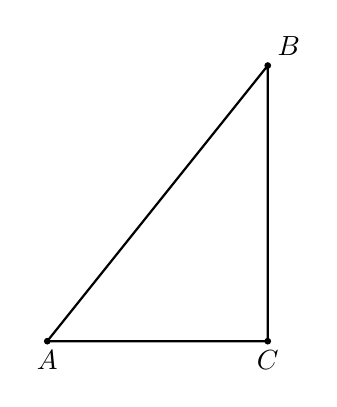
\begin{tikzpicture}[scale=0.7]
      \draw [thick](0,0)--(4,0)--(4,5)--(0,0);
      \draw [fill] (0,0) circle [radius=0.05] node[below]{$A$};
      \draw [fill] (4,0) circle [radius=0.05] node[below]{$C$};
      \draw [fill] (4,5) circle [radius=0.05] node[above right]{$B$};
      %\draw [color=blue] (0,0) ++(0.75,0) arc [start angle=0, end angle=70, radius=0.75];
      %\draw [color=blue] (4,0) ++(-0.22, 0.73) arc [start angle=110, end angle=180, radius=0.75];
      %\draw [thick] (0.8,3.1)--(1.2,2.9); %tick mark
      %\draw [thick] (2.8,2.9)--(3.2,3.1); %tick mark
      %\node [right] at (3.25,2.5){$x+7$};
      %\node [left] at (0.75,2.5){$2x+1$};
    \end{tikzpicture}
  \end{center}
    \begin{enumerate}
      \item $\displaystyle \sin A = \frac{5}{6.4} = 0.781$ \vspace{1cm}
      \item $\cos A =$ \vspace{1cm}
      \item $\tan A =$
    \end{enumerate}

    \item Given right $\triangle DEF$ with $DE=7, EF=3, DF=7.6$, $m\angle E=90^\circ$. Express each trig ratio as a fraction, then as a decimal to the nearest thousandth.
      \begin{center}
        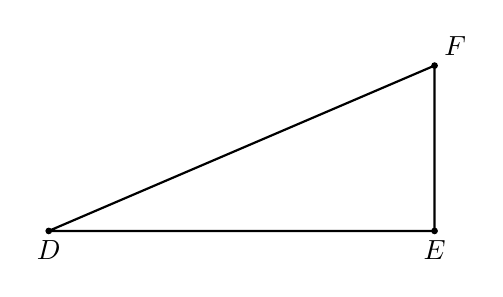
\begin{tikzpicture}[scale=0.7]
          \draw [thick](0,0)--(7,0)--(7,3)--(0,0);
          \draw [fill] (0,0) circle [radius=0.05] node[below]{$D$};
          \draw [fill] (7,0) circle [radius=0.05] node[below]{$E$};
          \draw [fill] (7,3) circle [radius=0.05] node[above right]{$F$};
          %\draw [color=blue] (0,0) ++(0.75,0) arc [start angle=0, end angle=70, radius=0.75];
          %\draw [color=blue] (4,0) ++(-0.22, 0.73) arc [start angle=110, end angle=180, radius=0.75];
          %\draw [thick] (0.8,3.1)--(1.2,2.9); %tick mark
          %\draw [thick] (2.8,2.9)--(3.2,3.1); %tick mark
          %\node [right] at (3.25,2.5){$x+7$};
          %\node [left] at (0.75,2.5){$2x+1$};
        \end{tikzpicture} \vspace{1cm}
      \end{center}
      \begin{multicols}{2}
        \begin{enumerate}
          \item $\sin F = $ \vspace{1cm}
          \item $\cos F =$ \vspace{1cm}
          \item $\tan F =$
          \item $\sin D = $ \vspace{1cm}
          \item $\cos D =$ \vspace{1cm}
          \item $\tan D =$

        \end{enumerate}
      \end{multicols}

      \newpage
  \subsubsection*{Classwork: Use a calculator for trig ratio}
    \item Express the result to the nearest thousandth.  \vspace{1cm}

      \begin{multicols}{2}
        \begin{enumerate}
          \item $\sin 30^\circ = $ \vspace{1cm}
          \item $\cos 45^\circ =$ \vspace{1cm}
          \item $\tan 60^\circ =$
          \item $\sin 57^\circ = $ \vspace{1cm}
          \item $\cos 23^\circ =$ \vspace{1cm}
          \item $\tan 81^\circ =$

        \end{enumerate}
      \end{multicols} \vspace{1cm}

      \item Given right $\triangle JKL$ with $\overline{JK} \perp \overline{KL}$, $JL=10$, $m\angle J=25^\circ$.
        \begin{center}
          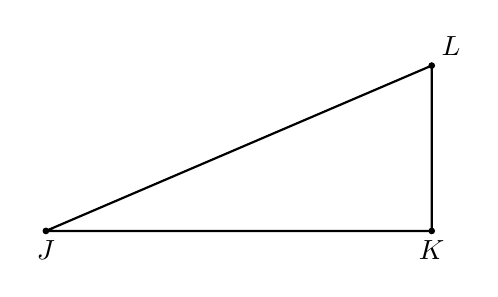
\begin{tikzpicture}[scale=0.7]
            \draw [thick](0,0)--(7,0)--(7,3)--(0,0);
            \draw [fill] (0,0) circle [radius=0.05] node[below]{$J$};
            \draw [fill] (7,0) circle [radius=0.05] node[below]{$K$};
            \draw [fill] (7,3) circle [radius=0.05] node[above right]{$L$};
            %\draw [color=blue] (0,0) ++(0.75,0) arc [start angle=0, end angle=70, radius=0.75];
            %\draw [color=blue] (4,0) ++(-0.22, 0.73) arc [start angle=110, end angle=180, radius=0.75];
            %\draw [thick] (0.8,3.1)--(1.2,2.9); %tick mark
            %\draw [thick] (2.8,2.9)--(3.2,3.1); %tick mark
            %\node [right] at (3.25,2.5){$x+7$};
            %\node [left] at (0.75,2.5){$2x+1$};
          \end{tikzpicture} \vspace{1cm}
        \end{center}
        \begin{enumerate}
          \item Find the length $JK$\\[3cm]
          \item Find the length $KL$
        \end{enumerate}

\end{enumerate}
\end{document}
